% preamble
\documentclass{tufte-book}

\usepackage[utf8]{inputenc}
\usepackage[T1]{fontenc}
\usepackage{lmodern}
\usepackage{amsmath}
\usepackage{amssymb}
\usepackage{amsthm}
\usepackage{mathtools}
\usepackage{empheq}
\usepackage{parskip}
\usepackage{hyperref}
\usepackage{pgfplots}
\usepackage{cleveref}
\usepackage{graphicx}
\usepackage{titlesec}

\pgfplotsset{compat=1.18}

\title{Undergraduate Mathematics I}
\author{London Wallace}
\date{2026}

\renewcommand{\chaptermark}[1]{\markboth{#1}{}}

\pagestyle{fancy}
\fancyhf{}
\fancyhead[RO]{\textbf{\textit{\leftmark} \quad \thepage}}
\renewcommand{\headrulewidth}{0pt}

\fancypagestyle{plain}{\fancyhf{}\renewcommand{\headrulewidth}{0pt}}

\setcounter{tocdepth}{2}

\newtheorem{theorem}{Theorem}

\titleformat{\part}[display]
  {\raggedright}
{\Large \allcaps{\partname \hspace{1em} \thepart}}
  {8pc}
  {\Huge \itshape}

\begin{document}

% title page and toc
\begin{titlepage}
	\raggedright {\Large \allcaps{London Wallace}}
	\par
	\vspace{8pc}
	{\itshape \Huge {Undergraduate Mathematics I}}
	{\tiny \allcaps {An Introduction to Calculus, Algebra, Analysis, and their Applications.}}
	\vfill
	{\small \allcaps {University of Western Australia}}
\end{titlepage}

\tableofcontents

\part{Prologue}
\fancyhead[LE]{\textbf{\thepage \quad \textit{Prologue}}}
\chapter{Notation}
\chapter{Numbers}
\chapter{Set Theory}
\chapter{Functions of Real Numbers}
\chapter{Complex Numbers}
\chapter{Proofs}
\part{Calculus}
\fancyhead[LE]{\textbf{\thepage \quad \textit{Calculus}}}
\chapter{Limits}
\chapter{Derivatives}
\chapter{Differentiation}
\chapter{Integrals}
\chapter{The Fundamental Theorem of Calculus}
\chapter{Integration Techniques}
\chapter{Inverse Functions}
\part{Mechanics}
\fancyhead[LE]{\textbf{\thepage \quad \textit{Mechanics}}}
\part{Multivariable Calculus}
\fancyhead[LE]{\textbf{\thepage \quad \textit{Multivariable Calculus}}}
\part{Electromagnetism and Waves}
\fancyhead[LE]{\textbf{\thepage \quad \textit{Electromagnetism, Waves, and Theoretical Mechanics}}}
\part{Linear Algebra}
\fancyhead[LE]{\textbf{\thepage \quad \textit{Linear Algebra}}}

%Chapter 1 - Foundations
\chapter{Foundations}

\newthought{Linear Algebra}, at least at this stage, is the study of linear functions, their behaviour and
interactions, where they live in space, and how they can be represented with matrices and determinants \cite{axler2015}.
The \emph{linear} in linear function refers to the fact that any variables, $x, y, z,$ etc, are never raised to any
power or multiplied together, only ever multiplied by scalars\sidenote{Scalars are numbers, real or complex. It soon becomes obvious why
	they are called scalars.} or added together. Geometrically this means that linear functions never curve. (\cref{fig:line})

Linear functions generally take the form:
\begin{equation*}
	y = mx + b
\end{equation*}
\begin{marginfigure}[+1cm]
	\begin{tikzpicture}
		\begin{axis}[
				width=\linewidth,
				height=4cm,
				axis lines=center,
				xlabel={$x$},
				ylabel={$y$},
				ticks=none,
				xmin=-2.5, xmax=2.5,
				ymin=-2.5, ymax=2.5,
			]
			\addplot[black, thick, samples=100, domain=-2:2] {(0.8*x)};
		\end{axis}
	\end{tikzpicture}
	\caption{A linear function.}
	\label{fig:line}
\end{marginfigure}
Where $m$ and $b$ are numbers, and $x$ and $y$ are variables. In this form, $m$ represents the \emph{slope} of the line,
how steep it appears on the plot, and $b$ represents the $y$-intercept, the point at which the line crosses the
vertical axis.

You can also define a line by the points it intersects (\cref{fig:line_from_points}). You only need two points to figure out the equation
representing a line. Imagine a line traveling through the points $(-1,-1)$ and $(1,2)$. The slope of this line, its
\emph{rise over run}, would be $y_2-y_1$ divided by $x_2-x_1$ (The height gained divided by the distance travelled),
and the $y$-intercept would be $y_{1,2}-mx_{1,2}$, obtained by rearranging the form we want the equation to take.

\begin{equation*}
	y=\left(\dfrac{y_2-y_1}{x_2-x_1}\right)x+\left(y_1-\left(\dfrac{y_2-y_1}{x_2-x_1}\right)x_1\right)
\end{equation*}
\begin{equation*}
	\implies y=\left(\dfrac{(2)-(-1)}{(1)-(-1)}\right)x+\left((-1)-\left(\dfrac{(2)-(-1)}{(1)-(-1)}\right)(-1)\right)
\end{equation*}
\begin{equation*}
	\implies y=\left(\dfrac{3}{2}\right)x+\left(\dfrac12\right)
\end{equation*}
\begin{marginfigure}[-8cm]
	\begin{tikzpicture}
		\begin{axis}[
				width=\linewidth,
				height=4cm,
				axis lines=center,
				xlabel={$x$},
				ylabel={$y$},
				ticks=none,
				xmin=-3, xmax=3,
				ymin=-3, ymax=3,
			]
			\addplot[only marks, mark=*, black] coordinates {(-1,-1) (1,2)};
			\addplot[black, thick, samples=100, domain=-2:2] {(1.5*x)+0.5};
		\end{axis}
	\end{tikzpicture}
	\caption{$(-1,-1)$ and $(1,2)$ and $y=1.5x+0.5$}
	\label{fig:line_from_points}
\end{marginfigure}
The middle line looks very complicated, but only due to my verbosity. They are just numbers.

\section{Vectors}

\newthought{Vectors are quantities with a magnitude and a direction}. They are used to represent things like force
or momentum. It does not make much sense, for example, just to say "the ball experiences a force of 5N", we must
add where the force is directed, 5N \emph{down}. Vectors are usually notated with an arrow above their name,
$\overrightarrow{\text{vector}}$.

\begin{marginfigure}
	\begin{tikzpicture}
		\begin{axis}[
				width=\linewidth,
				height=4cm,
				axis lines=center,
				xlabel={$x$},
				ylabel={$y$},
				ticks=none,
				xmin=-0.5, xmax=4,
				ymin=-0.5, ymax=4,
			]

			\draw[->, thick, black]
			(axis cs:0,0) -- (axis cs:2,2)
			node[above] {$\vec{u}=(2,2)$};

			\draw (axis cs:0.7,0) arc [start angle=0, end angle=45, radius=0.7]
			node[pos=0.5, right] {$\theta$};

			% Dotted line for height (vertical)
			\draw[dotted, thick] (axis cs:2,0) -- (axis cs:2,2);

			% Dotted line for length/width (horizontal)
			\draw[dotted, thick] (axis cs:0,2) -- (axis cs:2,2);

		\end{axis}
	\end{tikzpicture}
	\caption{Vectors can be defined both by the point they end on, and their length and angle from an axis.}
	\label{fig:vectors}
\end{marginfigure}

Vectors are usually written down just as a set of points, $\vec{u}=(2,2)$. This translates to "the vector \textbf{u}
starts at the origin $(0,0)$ and ends at the point $(2,2)$." From \cref{fig:vectors} we can see
that this vector forms a right triangle with base length 2, height 2 and, from the Pythagorean theorem, hypotenuse
$\sqrt{2^2+2^2} \approx 2.83$. The angle from the $x$ axis, $\theta$ is then $\cos^{-1}\left(\frac{2}{2.83}\right)=45^{\circ}$.

If this vector, $\vec{u}=(2,2)$, were being used to represent force, for example, the force would have a magnitude of
2.83N and a direction of $45^{\circ}$.

In three dimensions its slightly more complicated by much the same. The vector $\vec{r}=(2,2,2)$ starts at the origin,
goes to the point $(x,y,z)=(2,2,2)$ and stops. We now need two angles and its length to fully describe it, the angle
$\phi$ is the angle the projection of the vector on the $x-y$ plane makes with the $x$ axis, and the angle $\theta$
is the angle the vector makes with the $z$ axis.

To calculate $\phi$, you ignore the $z$ coordinate and pretend you just have a vector in 2 dimensions. Now you can
figure out its angle with the $x$ axis like we did above. Calculating $\theta$ is much the same, ignore the $x$
coordinate, and now you just have a $2D$ vector again! (\cref{fig:vector-3d})
The length of this vector $\vec{r}$ is just the Pythagorean theorem in 3 dimensions,
$|r|=\sqrt{x^2+y^2+z^2}=\sqrt{2^2+2^2+2^2} \approx 3.46$.

\begin{marginfigure}[-6cm]
	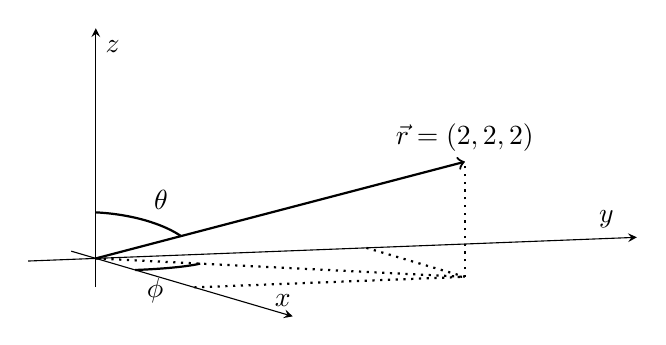
\begin{tikzpicture}
		\begin{axis}[
				width=\linewidth,
				height=6cm,
				view={70}{15},
				axis lines=center,
				ticks=none,
				xlabel={$x$}, ylabel={$y$}, zlabel={$z$},
				xlabel style={xshift=0pt,yshift=-3pt},
				xmin=-0.5, xmax=4,
				ymin=-0.5, ymax=4,
				zmin=-0.5, zmax=4,
			]

			% Vector u = (2, 0, 0)
			\draw[->, thick, black]
			(axis cs:0,0,0) -- (axis cs:2,2,2)
			node[above] {$\vec{r}=(2,2,2)$};

			\draw[dotted, thick] (axis cs:2,0,0) -- (axis cs:2,2,0);
			\draw[dotted, thick] (axis cs:0,2,0) -- (axis cs:2,2,0);
			\draw[dotted, thick] (axis cs:2,2,0) -- (axis cs:2,2,2);
			\draw[dotted, thick] (axis cs:0,0,0) -- (axis cs:2,2,0);

			\addplot3[domain=0:45, samples=20, samples y=0, domain y=0, thick, domain=0:45]
			({0.8*cos(x)}, {0.8*sin(x)}, {0})
			node[pos=0.5, below left] {$\phi$};

			\addplot3[domain=0:54.7, samples=20, samples y=0, thick]
			({0.8*sin(x)*cos(45)}, {0.8*sin(x)*sin(45)}, {0.8*cos(x)})
			node[pos=0.5, above right] {$\theta$};

		\end{axis}
	\end{tikzpicture}
	\caption{Vectors in $3D$ require 2 angles and a length.}
	\label{fig:vector-3d}
\end{marginfigure}

We can generalise this concept to as many dimensions as we want. We say a vector is an \emph{ordered n-tuple} of
numbers, which just means a list, \emph{n} items long\sidenote[][-1cm]{In $2D, n=2$. In $3D, n=3$. A $1D$ vector is just
	a number.}.
\begin{equation*}
	\vec{v}=(v_1,v_2,...,v_{n-1},v_n) \text{ where } v_{1-n} \text{ are numbers.}
\end{equation*}

\subsection{Vector Addition}

\newthought{Vectors can be added} by adding up their members. This produces another vector that, geometrically,
has an angle from the $x$ axis inbetween the angles of the two input vectors, with total length equal to the sum of
the lengths of each input vector
(\cref{fig:vector_addition}).
\begin{equation*}
	\overrightarrow{u+v}=\vec{u}+\vec{v}=(u_1+v_1,u_2+v_2,...,u_n+v_n)
\end{equation*}

\begin{marginfigure}[+1cm]
	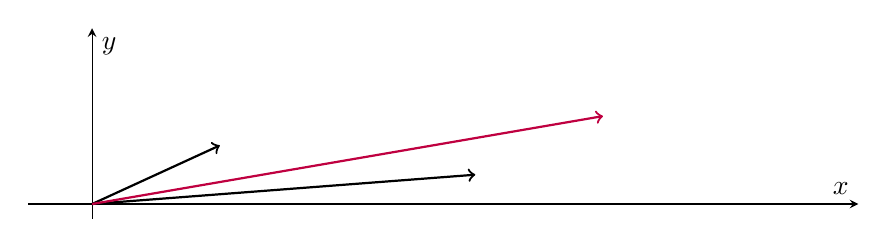
\begin{tikzpicture}
		\begin{axis}[
				width=\linewidth,
				height=4cm,
				axis lines=center,
				xlabel={$x$},
				ylabel={$y$},
				ticks=none,
				xmin=-0.5, xmax=6,
				ymin=-0.5, ymax=6,
			]
			\addplot[->, thick, black] coordinates {(0,0) (1,2)};
			\addplot[->, thick, black] coordinates {(0,0) (3,1)};
			\addplot[->, thick, purple] coordinates {(0,0) (4,3)};
		\end{axis}
	\end{tikzpicture}
	\caption{$\vec{u}=(1,2), \vec{v}=(3,1) \text{ and } \overrightarrow{u+v}=(4,3)$}
	\label{fig:vector_addition}
\end{marginfigure}

\subsection{Scalar Multiplication}

\newthought{Vectors are scaled} by multiplying them with a number. This produces a vector that points in the same
direction but is longer by whichever \emph{scaling factor} you multiplied by. This is achieved by distributing
the number to all the members of the vector.
\begin{equation*}
	\lambda \vec{u} = (\lambda u_1, \lambda u_2, ..., \lambda u_n) \text{ for some }\lambda \in \mathbb{R}
\end{equation*}

\subsection{Vector Multiplication}

\newthought{Vectors can be multiplied} in two ways; one that produces a number, and one that produces another vector.
The \emph{dot} product is the sum of the product of the respective members of two vectors of the same length.
\begin{equation*}
	\vec{u} \cdot \vec{v} = (u_1 \times v_1) + (u_2 \times v_2) + ... + (u_n \times v_n)
\end{equation*}
It represents how much of one vector \emph{goes} in the direction of another. This is particularly useful if
one of the vectors you are taking the dot product with is a unit vector\sidenote[][-4.5cm]{Unit vectors are vectors that travel
	along an axis and have length $1$, e.g $(1,0)$ and $(0,1)$ are the unit vectors of the $x-y$ plane. Unit vectors are denoted by a little
	hat. Traditionally, $\hat{\imath}, \hat{\jmath},\text{ and } \hat{k}$ represent the unit vectors in the
	$x, y, \text{ and }z$ directions, respectively.} since it tells you how much of a vector goes in the unit vector's
direction.

For example, if you have some vector representing force, $\vec{F}$, and you take its dot product with $\hat{\imath}$
you get the amount of force in the $x$ direction, its $x-$component.

\begin{marginfigure}
	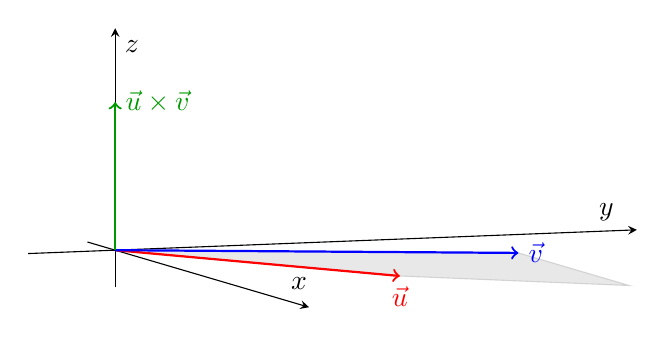
\begin{tikzpicture}
		\begin{axis}[
				width=\linewidth,
				height=6cm,
				view={70}{15},
				axis lines=center,
				ticks=none,
				xlabel={$x$}, ylabel={$y$}, zlabel={$z$},
				xmin=-0.5, xmax=3.5,
				ymin=-0.5, ymax=3,
				zmin=-0.5, zmax=3,
			]

			% Shaded plane spanned by u and v (parallelogram)
			\addplot3[
				fill=gray!30, opacity=0.6, draw=gray!50
			] coordinates {
					(0,0,0) (2,1,0) (3,2,0) (1,2,0) (0,0,0)
				};

			% Vector u = (2, 0, 0)
			\draw[->, thick, red]
			(axis cs:0,0,0) -- (axis cs:2,1,0)
			node[below] {$\vec{u}$};

			% Vector v = (1, 2, 0)
			\draw[->, thick, blue]
			(axis cs:0,0,0) -- (axis cs:1,2,0)
			node[right] {$\vec{v}$};

			% Cross product u x v = (0, 0, 4), drawn shorter for aesthetics
			\draw[->, thick, green!60!black]
			(axis cs:0,0,0) -- (axis cs:0,0,2)
			node[right] {$\vec{u} \times \vec{v}$};

		\end{axis}
	\end{tikzpicture}
	\caption{The cross product $\vec{u}\times\vec{v}$ is normal to the plane containing $\vec{u}$ and $\vec{v}$.}
	\label{fig:cross_product}
\end{marginfigure}

\newthought{The cross product} of two vectors produces another vector. Geometrically, this new vector is perpendicular to
the plane containing the input vectors. We say that the cross product of two vectors $\vec{u}$ and $\vec{v}$,
$\vec{u} \times \vec{v}$ is \emph{normal} to the surface containing them (\cref{fig:cross_product}). If you hold your right hand out in front
of you in the shape of a gun, leave your pointer finger in the direction of $\vec{u}$ and bend your middle finger
to the direction of $\vec{v}$, your pointer and middle fingers are two vectors that form a plane. Your thumb
pointing up or down is normal to that plane. If your pointer was $\vec{u}$ and your middle finger $\vec{v}$ then your
thumb would be their cross product, $\vec{u} \times \vec{v}$ (\cref{fig:right-hand-rule}).

\begin{marginfigure}
	\centering
	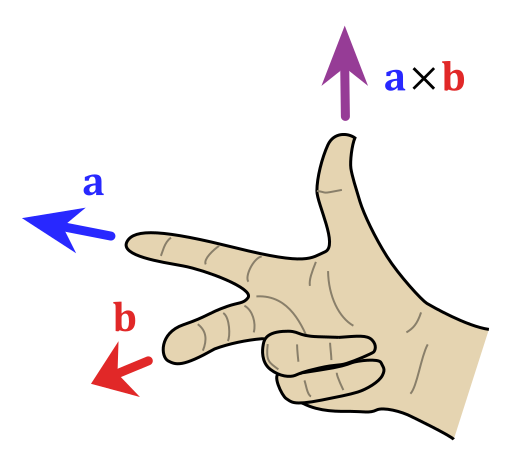
\includegraphics[width=\linewidth]{Right_hand_rule_cross_product.png}
	\caption{The right hand rule for cross products.}
	\label{fig:right-hand-rule}
\end{marginfigure}

That is, in fact, the definition of the cross product:
\begin{equation*}
	\vec{u} \times \vec{v} = |u| \cdot |v| \sin(\theta) \vec{n}
\end{equation*}
Where $|u|$ is the magnitude, or length, of $\vec{u}$, $\theta$ is the angle between $\vec{u}$ and $\vec{v}$, and
$\vec{n}$ is the unit normal vector to the plane containing $\vec{u}$ and $\vec{v}$, determined via the right hand
rule.

\newthought{The cross product satisfies the following rules, or axioms.}

\begin{enumerate}
	\item The cross product is \textbf{anticommutative}.
	      \begin{equation*}
		      \vec{u} \times \vec{v} = - (\vec{v} \times \vec{u})
	      \end{equation*}
	      Going back to the right hand rule from earlier, if you put your left hand out in front of you and try to make the same
	      shape with your pointer and middle fingers as is on your right hand, the only way to do this is to have your thumb
	      pointing down.

	\item The cross product is \textbf{distributive over addition}.
	      \begin{equation*}
		      \vec{u} \times (\vec{v} + \vec{r}) = \vec{u} \times \vec{v} + \vec{u} \times \vec{r}
	      \end{equation*}

	\item Scalars can be factored out.
	      \begin{equation*}
		      (\lambda \cdot \vec{u}) \times \vec{v} = \lambda(\vec{u} \times \vec{v})
	      \end{equation*}

	\item A vector \emph{dotted} with a cross product of itself is 0.
	      \begin{equation*}
		      \vec{u} \cdot (\vec{u} \times \vec{v}) = 0
	      \end{equation*}
	      Recall from the definition of a dot product that it represents the amount of one vector that goes in the direction of
	      another. If a cross product is perpendicular to both its input vectors then none of the input vector will \emph{go} in
	      the direction of the cross product, so by definition their dot product must be 0.
\end{enumerate}

\begin{marginfigure}[-0cm]
	\centering
	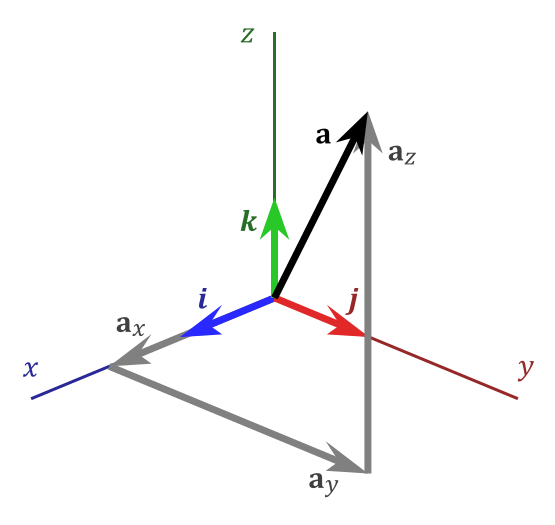
\includegraphics[width=0.98\linewidth]{3D_Vector.png}
	\caption{The unit vectors, $\hat{\imath}, \hat{\jmath}, \hat{k}$ and the components of $\vec{a}: \vec{a}_x, \vec{a}_y,
			\vec{a}_z$}
	\label{fig:3d_vectors}
\end{marginfigure}

The standard unit vectors $\hat{\imath}, \hat{\jmath}, \hat{k}$ satisfy the following equalities:
\begin{equation*}
	\hat{\imath} \times \hat{\jmath} = \hat{k}
\end{equation*}
\begin{equation*}
	\hat{\jmath} \times \hat{k} = \hat{\imath}
\end{equation*}
\begin{equation*}
	\hat{k} \times \hat{\imath} = \hat{\jmath}
\end{equation*}

And by anticommutivity:
\begin{equation*}
	\hat{\jmath} \times \hat{\imath} = -\hat{k}
\end{equation*}
\begin{equation*}
	\hat{k} \times \hat{\jmath} = -\hat{\imath}
\end{equation*}
\begin{equation*}
	\hat{\imath} \times \hat{k} = -\hat{\jmath}
\end{equation*}

This implies that:
\begin{equation*}
	\hat{\imath} \times \hat{\imath} = \hat{\jmath} \times \hat{\jmath} = \hat{k} \times \hat{k} = \textbf{0}
\end{equation*}

Since we also know that any vector $\vec{a}$ can be represented by \\
$a_1\hat{\imath}+a_2\hat{\jmath}+a_3\hat{k}$
(\cref{fig:3d_vectors}). This is enough to derive\sidenote{Much simpler methods
	will be discussed later, however it is important to understand the derivation from the axioms.}:
\begin{equation*}
	\vec{a} \times \vec{b} = (a_1\hat{\imath}+a_2\hat{\jmath}+a_3\hat{k}) \times (b_1\hat{\imath}+b_2\hat{\jmath}+b_3\hat{k}) =
\end{equation*}
\begin{equation*}
	a_1b_1(\hat{\imath}\times\hat{\imath})+a_1b_2(\hat{\imath}\times\hat{\jmath})+a_1b_3(\hat{\imath}\times\hat{k}) +
\end{equation*}
\begin{equation*}
	a_2b_1(\hat{\jmath}\times\hat{\imath})+a_2b_2(\hat{\jmath}\times\hat{\jmath})+a_2b_3(\hat{\jmath}\times\hat{k}) +
\end{equation*}
\begin{equation*}
	a_3b_1(\hat{k}\times\hat{\imath})+a_3b_2(\hat{k}\times\hat{\jmath})+a_3b_3(\hat{k}\times\hat{k})
\end{equation*}
\begin{equation*}
	= a_1b_2(\hat{k}) - a_1b_3(\hat{\jmath}) - a_2b_1(\hat{k}) + a_2b_3(\hat{\imath}) + a_3b_1(\hat{\jmath}) - a_3b_2(\hat{\imath})
\end{equation*}
\begin{equation*}
	=(a_2b_3-a_3b_2)\hat{\imath} + (a_3b_1-a_1b_3)\hat{\jmath} + (a_1b_2-a_2b_1)\hat{k}
\end{equation*}

\newthought{Vectors can be multiplied and added in these ways to form a vector space},
which will be defined properly later.
Vectors and vector spaces are principle objects of study in linear algebra. Collections of vectors are called
\emph{matrices}.

\section{Matrices}

\newthought{Matrices are ordered arrays of numbers.} An $m \times n$ matrix has $m$ rows and $n$ columns.
\[
	\begin{bmatrix}
		a_{11} & a_{12} & \cdots & a_{1n} \\
		a_{21} & a_{22} & \cdots & a_{2n} \\
		a_{31} & a_{32} & \cdots & a_{3n} \\
		\vdots & \vdots & \ddots & \vdots \\
		a_{m1} & a_{m2} & \cdots & a_{mn}
	\end{bmatrix}
\]

\subsection{Matrix Addition}
\newthought{Matrices can be added} if they are the same size and square. To add matrices simply add each element
to the corresponding element in the other matrix.
\[
	\begin{bmatrix}
		a & c \\
		b & d
	\end{bmatrix}
	+
	\begin{bmatrix}
		e & g \\
		f & h
	\end{bmatrix}
	=
	\begin{bmatrix}
		a+e & c+g \\
		b+f & d+h
	\end{bmatrix}
\]

\subsection{Matrix Scalar Multiplication}
Like vectors, scalars can just be distributed to each element in a matrix.
\begin{equation*}
	\lambda \cdot
	\begin{bmatrix}
		a & c \\
		b & d
	\end{bmatrix}
	=
	\begin{bmatrix}
		\lambda a & \lambda c \\
		\lambda b & \lambda d
	\end{bmatrix}
\end{equation*}

\subsection{Matrix Multiplication}
\newthought{To multiply two matrices}, you take the dot product of the rows of the first matrix with the columns of the
second and \emph{distribute} the results to the new matrix; i.e. first row $\cdot$ first column goes in the $(1,1)$
position and first row $\cdot$ second column goes in the $(1,2)$ position and so on. Thus the number of rows and columns
must be equal; i.e. you can only multiply $m \times n$ matrices with $n \times p$ matrices. The result of a matrix
\textbf{A} times a matrix \textbf{B} is called the matrix product \textbf{AB}.
\begin{equation*}
	\begin{bmatrix}
		a_1 & a_3 & a_5 \\
		a_2 & a_4 & a_6
	\end{bmatrix}
	\times
	\begin{bmatrix}
		b_1 & b_4 \\
		b_2 & b_5 \\
		b_3 & b_6
	\end{bmatrix}
	=
\end{equation*}
\begin{equation*}
	\begin{bmatrix}
		(a_1b_1+a_3b_2+a_5b_3) & (a_1b_4+a_3b_4+a_5b_6) \\
		(a_2b_1+a_4b_2+a_6b_3) & (a_2b_4+a_4b_5+a_6b_6)
	\end{bmatrix}
\end{equation*}
\newthought{Matrix multiplication satisfies the following axioms:}
\begin{enumerate}
	\item Matrix multiplication is non-commutative\sidenote{Recall an operation is commutative if given two elements
		      \textbf{A} and \textbf{B} such that the product \textbf{AB} is defined, then \textbf{BA} is also defined and
		      \textbf{AB} $=$ \textbf{BA}}.

	      If \textbf{A} and \textbf{B} are matrices of size $m \times n$ and $p \times q$ respectively then the matrix
	      product \textbf{AB} is only defined if $n=p$ and \textbf{BA} only defined if $m=q$. If $n=p \ne m=q$ then both products
	      are defined but not the same size so can't be equal and so the only case when both products are defined and could be
	      equal is when $m=n=p=q$; i.e both matrices are square and the same size. Even in this case \textbf{AB} generally does
	      not equal \textbf{BA}. For example:
	      \begin{equation*}
		      \begin{bmatrix}
			      0 & 1 \\
			      0 & 0
		      \end{bmatrix}
		      \times
		      \begin{bmatrix}
			      0 & 0 \\
			      1 & 0
		      \end{bmatrix}
		      =
		      \begin{bmatrix}
			      1 & 0 \\
			      0 & 0
		      \end{bmatrix}
	      \end{equation*}
	      but:

	      \begin{equation*}
		      \begin{bmatrix}
			      0 & 0 \\
			      1 & 0
		      \end{bmatrix}
		      \times
		      \begin{bmatrix}
			      0 & 1 \\
			      0 & 0
		      \end{bmatrix}
		      =
		      \begin{bmatrix}
			      0 & 0 \\
			      0 & 1
		      \end{bmatrix}
	      \end{equation*}

	      Only when one of the matrices is the identity matrix\sidenote{Defined below.}, or both are square diagonal
	      matrices\sidenote{A matrix with all zeroes other than the main top-left to bottom-right diagonal.}, is
	      \textbf{AB} $=$ \textbf{BA}.

	\item Matrix multiplication is distributive over addition.

	      Given 4 matrices, \textbf{A}, \textbf{B}. \textbf{C}, and \textbf{D} with sizes $m \times n$, $n \times p$, $n \times p$
	      and $p \times q$, one has both left and right distributivity:
	      \begin{equation*}
		      \textbf{A}(\textbf{B} + \textbf{C}) = \textbf{AB} + \textbf{AC}
	      \end{equation*}
	      \begin{equation*}
		      (\textbf{B} + \textbf{C})\textbf{D} = \textbf{BD} + \textbf{CD}
	      \end{equation*}

	\item Matrix multiplication is associative \textbf{iff} given 3 matrices \textbf{A}, \textbf{B}, and \textbf{C},
	      the number of columns in \textbf{A} equals the number of rows in \textbf{B}, and the number of columns in
	      \textbf{B} equals the number of rows in \textbf{C}. \textbf{Iff} that is the case:
	      \begin{equation*}
		      (\textbf{AB})\textbf{C} = \textbf{A}(\textbf{BC})
	      \end{equation*}

	\item If the product \textbf{AB} is defined and $c \in \mathbb{R}$ then:
	      \begin{equation*}
		      c(\textbf{AB})=(c\textbf{A})\textbf{B} \text{ and } (\textbf{AB})c = \textbf{A}(\textbf{B}c)
	      \end{equation*}
\end{enumerate}

\subsection{The Identity Matrix}

\newthought{The identity matrix} is the special matrix \textbf{I}, with the property that any other matrix \textbf{A}
multiplied by it is unchanged. This property is known in mathematics as the \emph{multiplicative identity}.
\begin{equation*}
	\textbf{AI} = \textbf{IA} = \textbf{A}
\end{equation*}
It is a square diagonal matrix with its main diagonal all ones:
\begin{equation*}
	\begin{bmatrix}
		1      & 0      & 0      & \cdots & 0      \\
		0      & 1      & 0      & \cdots & 0      \\
		0      & 0      & 1      & \cdots & 0      \\
		\vdots & \vdots & \vdots & \ddots & \vdots \\
		0      & 0      & 0      & \cdots & 1
	\end{bmatrix}
\end{equation*}
Its size can be whatever is required for the multiplicative identity to hold.
\section{Summary}

The principle objects of study in linear algebra\sidenote{In this first pass.} are linear functions, or functions
of several variables where no variable is raied to any power, the vector, which is an \emph{ordered n-tuple} of numbers
usually representing some quantity with a magnitude and direction, the way vectors interact to form \emph{spaces}
through addition and multiplication, matrices, which are collections of vectors in an array, and the way matrices
interact with each other. We will explore how the properties briefly explained here are useful for solving problems
and see what structures follow from these few simple rules.

%Chapter 2 - Systems of Linear Equations
\chapter{Systems of Linear Equations}

\newthought{The systematic solving} of systems of equations is a necessary skill for anyone wishing to study linear
algebra. Many problems in this field can be reduced to a system of linear equations, and so solving them
algorithmically is crucial.

\newthought{A linear equation} is an equation of the form:
\begin{equation*}
	x+2y=4
\end{equation*}
\marginnote[-1cm]{This is the same as the above $y=mx+b$. In this case $y=-\frac12 x + 2$.}
A \emph{system} of linear equations, then, is a set of linear equations considered together:
\begin{equation*}
	x+2y=4
\end{equation*}
\begin{equation*}
	x-y=1
\end{equation*}
\begin{marginfigure}[-0cm]
	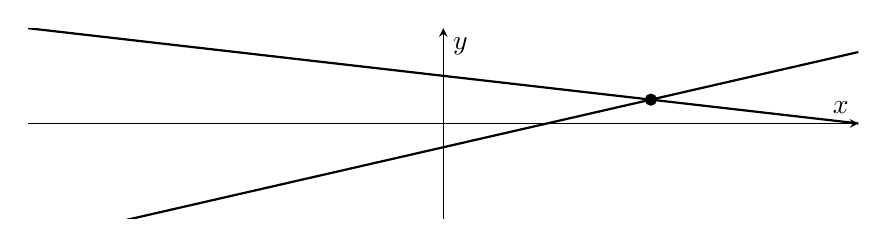
\begin{tikzpicture}
		\begin{axis}[
				width=\linewidth,
				height=4cm,
				axis lines=center,
				xlabel={$x$},
				ylabel={$y$},
				ticks=none,
				xmin=-4, xmax=4,
				ymin=-4, ymax=4,
			]
			\addplot[only marks, mark=*, black] coordinates {(2,1)};
			\addplot[black, thick, samples=100, domain=-4:4] {(-0.5*x)+2};
			\addplot[black, thick, samples=100, domain=-4:4] {x-1};
		\end{axis}
	\end{tikzpicture}
	\caption{$x+2y=4$, $x-y=1$ and their solution, $(2,1)$.}
	\label{fig:simple_sle}
\end{marginfigure}
Which is a system of two equations in two unknowns (\cref{fig:simple_sle}). You can have any number of equations in any number of unknowns
but for there to be a unique solution, you at least need to have as many equations as you have unknowns. When we have
$n$ unknowns, we generally write linear equations as:
\begin{equation*}
	a_1x_1+a_2x_2+a_3x_3+\cdots+a_nx_n=m \text{ | } a_{1-n},m \in \mathbb{R}, n \in \mathbb{N}.
\end{equation*}

\section{Solutions to Systems of Linear Equations}

\newthought{A solution} to a system of linear equations is any set of points $(x_1,x_2,\cdots,x_n)$ which satisfy every
equation in the system. The system presented above has a unique solution at $(2,1)$, but this is not always the case.
Consider the simple system (\cref{fig:sle_no_solution}):

\begin{marginfigure}[-2cm]
	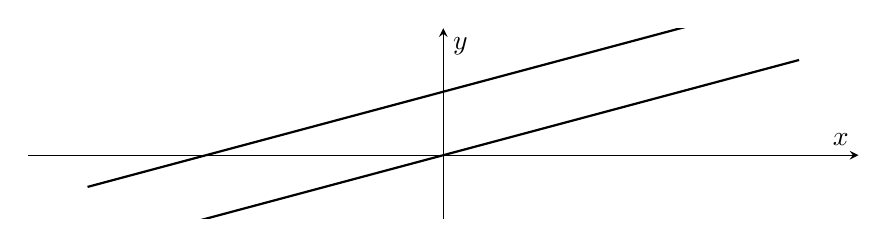
\begin{tikzpicture}
		\begin{axis}[
				width=\linewidth,
				height=4cm,
				axis lines=center,
				xlabel={$x$},
				ylabel={$y$},
				ticks=none,
				xmin=-3.5, xmax=3.5,
				ymin=-2, ymax=4,
			]
			\addplot[black, thick, samples=100, domain=-3:3] {x};
			\addplot[black, thick, samples=100, domain=-3:3] {x+2};
		\end{axis}
	\end{tikzpicture}
	\caption{The lines $y-x=0$ and $y-x=2$ are parallel and thus have no solution.}
	\label{fig:sle_no_solution}
\end{marginfigure}

\begin{equation*}
	y-x=0
\end{equation*}
\begin{equation*}
	y-x=2
\end{equation*}
The equations in this system are parallel and will never meet, thus there \emph{can't} be a solution.

The system below doesn't have a unique solution for a very different reason.
\begin{equation*}
	y-x=2
\end{equation*}
\begin{equation*}
	2y-2x=4
\end{equation*}
Notice, we can divide both sides of the second equation by 2, leaving us with the first equation. These two lines
are the same and so there are infinitely many solutions, every point on the line $y-x=2$.

Now, imagine you knew three equations in two unknowns (\cref{fig:three-sle-no-solution}):
\begin{align*}
	2x-y & = 1  \\
	x+y  & = 2  \\
	x-2y & = -2
\end{align*}
There is no solution of points $(x,y)=(a,b)$ that satisfies every equation, so the system has no solution.
Just because you know more equations than unknowns, that does not guarantee that a solution exists. Can you conceive
of a way to make this system have a solution? \sidenote{Shift the blue line down a bit?}
\begin{marginfigure}[-8cm]
	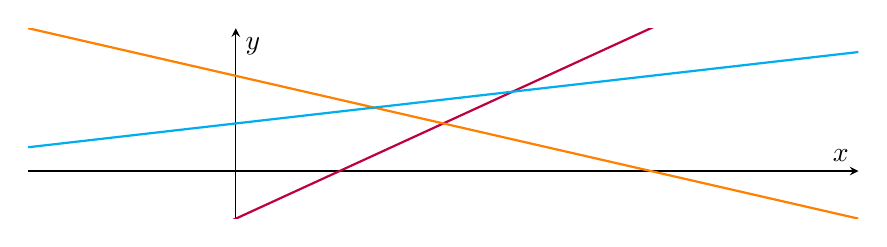
\begin{tikzpicture}
		\begin{axis}[
				width=\linewidth,
				height=4cm,
				axis lines=center,
				xlabel={$x$},
				ylabel={$y$},
				ticks=none,
				xmin=-1, xmax=3,
				ymin=-1, ymax=3,
			]
			\addplot[purple, thick, samples=100, domain=-1:3] {(2*x)-1};
			\addplot[orange, thick, samples=100, domain=-1:3] {2-x};
			\addplot[cyan, thick, samples=100, domain=-1:3] {(0.5*x)+1};
		\end{axis}
	\end{tikzpicture}
	\caption{The plots of $2x-y=1, x+y=2$ and $x-2y=-2$ never meet a single point.}
	\label{fig:three-sle-no-solution}
\end{marginfigure}

That is the case for \emph{every} system of linear equations, they either have no solutions, a unique solution or
infinitely many solutions. The intuition for each is that the lines never cross, all cross at the same point, or are
they same line. If a solution exists, we say the system is \emph{consistent}. If one does not exist, we say it
is \emph{inconsistent}.

\newthought{In three dimensions} linear equations form a plane. Consider the equation $x + y + z = 1$
(\cref{fig:simple-plane}).
It is the plane of all points $z$ that satisfy $z=1-x-y$. It is still possible to reason geometrically about linear
equations in three dimensions, but beyond that it is impossible. We therefore need to develop \emph{algebraic} methods
of understanding these systems, not just geometric.

Imagine you only know two equations in three unknowns:
\begin{align*}
	x+y+z & = 1 \\
	x-y-z & = 1
\end{align*}
\begin{marginfigure}[-3cm]
	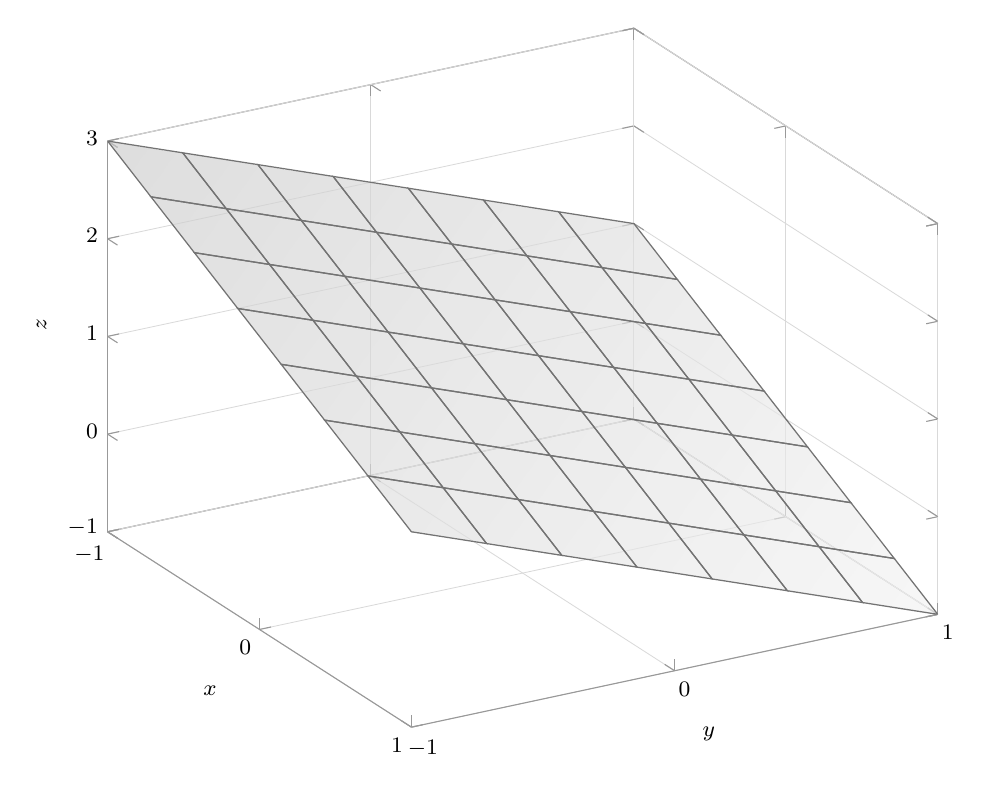
\begin{tikzpicture}
		\begin{axis}[
				width=\linewidth,
				view={60}{30},
				xlabel={$x$},
				ylabel={$y$},
				zlabel={$z$},
				xtick={-1,0,1},
				ytick={-1,0,1},
				ztick={-1,0,1,2,3},
				xmin=-1, xmax=1,
				ymin=-1, ymax=1,
				zmin=-1, zmax=3,
				tick style={thin, color=black!40},
				axis line style={thin, color=black!40},
				tick label style={font=\footnotesize},
				label style={font=\footnotesize\itshape},
				grid=major,
				grid style={line width=0.3pt, draw=black!15},
				axis background/.style={fill=none},
			]
			% Shaded surface
			\addplot3[
				surf,
				shader=interp,
				colormap={blueplane}{
						color=(black!5) color=(black!20)
					},
				opacity=0.65,
				domain=-1:1,
				y domain=-1:1,
				samples=30,
			]
			{ 1 - x - y };

			% Crisp wireframe overlay
			\addplot3[
				mesh,
				draw=black!55,
				line width=0.45pt,
				domain=-1:1,
				y domain=-1:1,
				samples=8,
			]
			{ 1 - x - y };

		\end{axis}
	\end{tikzpicture}
	\caption{The plane $x + y + z = 1$.}
	\label{fig:simple-plane}
\end{marginfigure}
Each of these equations defines a plane and since those planes are clearly not parallel, they will meet in a line.
Every point along that line will be a solution to this system.

One way of describing a system like this is to chose one of the variables to be free. If we chose $z$ to be free, the
first equation becomes $z=1-x-y$. We can then solve for the set of solutions by substituting this equation into the
other:
\begin{align*}
	x-y-(1-x-y) & = 1                                           \\
	2x          & = 2                                           \\
	x           & = 1 \text{ can now be used to solve for $y$.} \\
	1 + y + z   & = 1                                           \\
	y           & = -z
\end{align*}
So a full solution to this system would be:
\begin{equation*}
	S=\{(1,-z,z)\text{ | }z \in \mathbb{R}\}
\end{equation*}
Which means for any real number $z$, say $z=3$, there is a solution $(1,-z,z)=(1,-3,3)$ that satisfies both equations
in the system.

\section{Algorithmically Solving Systems of Linear Equations}

\newthought{An algorithm} is a set of instructions for solving a specific problem that works every time. In the case
of systems of linear equations, the algorithm is called \emph{Gauss-Jordan Elimination} and involves altering the
system in some way to make the solutions trivially obvious.

\subsection{Building the Augmented Matrix}

If you know $m$ equations in $n$ unknowns with $n,m \in \mathbb{N}$ and $a_n,k_n \in \mathbb{R}$:
\begin{align*}
	a_1x_1+a_2x_2+a_3x_3+\cdots+a_nx_n & = k_1 \\
	b_1x_1+b_2x_2+b_3x_3+\cdots+b_nx_n & = k_2 \\
	c_1x_1+c_2x_2+c_3x_3+\cdots+c_nx_n & = k_3 \\
	\vdots                                     \\
	m_1x_1+m_2x_2+m_3x_3+\cdots+m_nx_n & = k_m \\
\end{align*}
Then, following from the rules of matrix multiplication discussed in Chapter 1, you can build three matrices,
\textbf{A}, \textbf{x}, and \textbf{B} such that:
\begin{equation*}
	\textbf{Ax}=\textbf{B}
\end{equation*}
Where \textbf{A} is a $m \times n$ matrix containing all the coefficients $a_{1 \to n} \to m_{1 \to n}$,
\textbf{x} is a $n \times 1$ matrix containing all the variables $x_{1 \to n}$ and \textbf{B} is a
$m \times 1$ matrix containing all the scalars $k_{1 \to m}$:
\begin{equation*}
	\begin{bmatrix}
		a_1    & a_2    & \cdots & a_n    \\
		b_1    & b_2    & \cdots & b_n    \\
		\vdots & \vdots & \ddots & \vdots \\
		m_1    & m_2    & \cdots & m_n
	\end{bmatrix}
	\begin{bmatrix}
		x_1    \\
		x_2    \\
		\vdots \\
		x_n
	\end{bmatrix}
	=
	\begin{bmatrix}
		k_1    \\
		k_2    \\
		\vdots \\
		k_m
	\end{bmatrix}
\end{equation*}

This notation is quite a lot to write out every time you want to solve a system of linear equations. Generally, when
solving systems of linear equations by hand we build an \emph{augmented matrix} with the coefficients on the left,
and answers on the right; with the vertical line representing the "$\times \textbf{ x } =$" statement:
\[
	\left[
		\begin{array}{cccc|c}
			a_1    & a_2    & \cdots & a_n    & k_1    \\
			b_1    & b_2    & \cdots & b_n    & k_2    \\
			\vdots & \vdots & \ddots & \vdots & \vdots \\
			m_1    & m_2    & \cdots & m_n    & k_m
		\end{array}
		\right]
\]
It's done in this way because it makes the arithmetic of the following sections much easier to compute.
\subsection{Elementary Row Operations}

\newthought{Elementary Row Operations} are operations applied to the equations in a system of linear equations
to transform them into a simpler, but equivalent, system\sidenote{Equivalent meaning they have the same solution.}.
This is done because the resultant system is trivially easy to solve. Gauss-Jordan elimination, then, is just a
method for applying these operations that results in the same trivial system every time.

\newthought{They are:}
\begin{enumerate}
	\item Interchanging the order of equations.
	\item Multiplying an equation by a scalar.
	\item Adding a scalar multiple of one equation to another.
\end{enumerate}
\vspace{\baselineskip}
\begin{theorem}
	Let S be a system of linear equations and T be the resultant set of linear equations after applying
	arbitrary elementary row operations to S. The solution set of S equals the solution set of T.
\end{theorem}
\textit{Proof:}
You should not need any convincing that the first two row operations do not alter the solution of the system. The third
operation, however, requires some attention.
\newthought{Let} $S$ be the set of linear equations $E_1 \to E_n$:
\begin{equation*}
	S = \{E_1,E_2,E_3,\cdots,E_n\}
\end{equation*}
\newthought{Let} $E_i$ and $E_j \in S$:
\begin{align*}
	E_i & = a_{1i}x_1+a_{2i}x_2+\cdots+a_{ni}x_n \\
	E_j & = a_{1j}x_1+a_{2j}x_2+\cdots+a_{nj}x_n
\end{align*}
\newthought{Let} T be the set of linear equations that results from the addition of $k \cdot E_j$ to $E_i$:
\begin{equation*}
	T = \{E_1, E_2,\cdots, E'_i, E_j, \cdots, E_n \}
\end{equation*}
\newthought{Then} the only difference between $S$ and $T$ is $E'_i$:
\begin{equation*}
	E'_i = (a_{1i}+ka_{1j})x_1+(a_{2i}+ka_{2j})x_2+\cdots+(a_{ni}+ka_{nj})x_n = E_i+kE_j
\end{equation*}
\newthought{Let} $s$ be a solution to $S$:
\begin{equation*}
	s=(s_1,s_2,\cdots,s_n) \text{ | } s_i \in \mathbb{R}
\end{equation*}
\newthought{Then} check if $s$ is a solution to $T$:
\begin{align*}
	E'_i & = (a_{1i}+ka_{1j})s_1+(a_{2i}+ka_{2j})s_2+\cdots+(a_{ni}+ka_{nj})s_n             \\
	     & = a_{1i}s_1+ka_{1j}s_1+a_{2i}s_2+ka_{2j}s_2+\cdots+a_{ni}s_n+ka_{nj}s_n          \\
	     & \text{ which when grouped: }                                                     \\
	     & = (a_{1i}s_1+a_{2i}s_2+\cdots+a_{ni}s_n)+k(a_{1j}s_1+a_{2j}s_2+\cdots+a_{nj}s_n) \\
	     & = E_i + kE_j
\end{align*}
\newthought{So} any solution to $S$ is a solution to $T$ but we still need to check that any solution to $T$ is a
solution to $S$.
\newthought{If} a vector exists that satisfies all equations in $T$ then it necessarily satisfies $E_i+kE_j$ and
$E_j$. Therefore it also satisfies $E_i$ since:
\begin{equation*}
	E_i + kE_j + (-kE_j) = E_i
\end{equation*}
\newthought{Thus} any solution to $T$ is also a solution to $S$ and the theorem holds. \qed

\subsection{Gauss-Jordan Elimination}

\newthought{Gauss-Jordan Eliminiation} is an algorithm for applying elementary row operations to augmented
matrices\sidenote{The system doesn't \emph{need} to be represented as an augmented matrix, it just makes
	it easier.} to transform them into a trivial-to-solve system.

\newthought{Reduced Row Echelon Form} is the final result of Gauss-Jordan Elimination. An augmented matrix is in
reduced row echelon form if:
\begin{enumerate}
	\item Any rows of all zeroes occur in the last row(s), and,
	\item The first non-zero entry\sidenote{The first non-zero entry is called the leading entry.} of each row is
	      \emph{strictly to the right} of the first non-zero entry of the row above, and,
	\item The first non-zero entry of each row is equal to one.
\end{enumerate}

\newthought{In words}, Gauss-Jordan Elimination is carried out as follows: Let \textbf{A} be an $m \times n$ matrix.
At each stage in the algorithm, a particular entry of the matrix, called the \emph{pivot point} is being processed,
and the steps of the algorithm depend on the value of this pivot.
\begin{enumerate}
	\item Let the \emph{pivot point} be the top-left $(1,1)$ entry of the matrix. If this entry is 0, then interchange it
	      with the row whose first entry is closest to zero. To make the process easier, if this entry is not 1, but
	      there is a row with first entry equal to 1, interchange those two rows.
	\item Divide the first row by the value of the first entry such that the first entry becomes 1.
	\item Add and subtract as necessary the first row to other rows such that the first entry of every other row becomes
	      0.
	\item Move the pivot point down and to the right 1 unit, i.e. to the $(2,2)$ position of the matrix. If this entry
	      is 0, then interchange rows other than the first row, such that this entry is non-zero.
	\item Divide the second row by the value of its second entry, such that it becomes 1.
	\item Repeat steps 3-5 with respect to the new shifted pivot point each time until the matrix is as close to the
	      identity matrix as possible.
\end{enumerate}
This algorithm laid out in words is quite difficult to understand, so here is an example: The system (\cref{fig:three-sle}):
\begin{align*}
	2x-y   & = 1  \\
	x + y  & = 2  \\
	x - 2y & = -1
\end{align*}
\begin{marginfigure}[-0cm]
	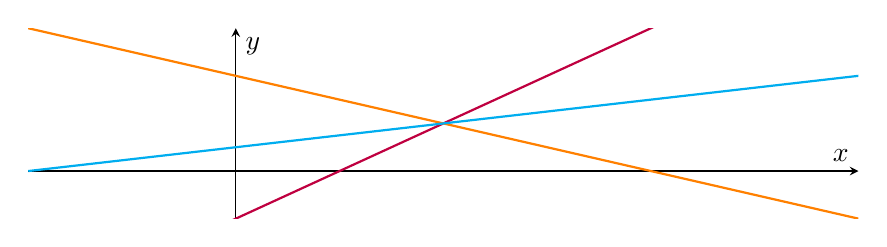
\begin{tikzpicture}
		\begin{axis}[
				width=\linewidth,
				height=4cm,
				axis lines=center,
				xlabel={$x$},
				ylabel={$y$},
				ticks=none,
				xmin=-1, xmax=3,
				ymin=-1, ymax=3,
			]
			\addplot[purple, thick, samples=100, domain=-1:3] {(2*x)-1};
			\addplot[orange, thick, samples=100, domain=-1:3] {2-x};
			\addplot[cyan, thick, samples=100, domain=-1:3] {(0.5*x)+(0.5)};
		\end{axis}
	\end{tikzpicture}
	\caption{The plots of $2x-y=1, x+y=2$ and $x-2y=-1$.}
	\label{fig:three-sle}
\end{marginfigure}
Is represented by the augmented matrix:
\begin{equation*}
	\left[
		\begin{array}{cc|c}
			2 & -1 & 1  \\
			1 & 1  & 2  \\
			1 & -2 & -1
		\end{array}
		\right]
\end{equation*}
The first pivot point is the top left entry:
\begin{equation*}
	\left[
		\begin{array}{cc|c}
			\boxed{2} & -1 & 1  \\
			1         & 1  & 2  \\
			1         & -2 & -1
		\end{array}
		\right]
\end{equation*}
Interchange rows 1 and 2 so that the top left entry is 1.\sidenote{The $\iff$ is used to indicate when elementary
	row operations have been applied. $R_1 \iff R_2$ means $R_1$ becomes $R_2$. $R_2 \iff R_2 - 2R_1$ means $R_2$
	becomes itself minus 2 times $R_1$.}
\begin{equation*}
	\left[
		\begin{array}{cc|c}
			\boxed{1} & 1  & 2  \\
			2         & -1 & 1  \\
			1         & -2 & -1
		\end{array}
		\right]
	\begin{array}{l}
		R_1 \iff R_2 \\
		R_2 \iff R_1 \\
		\\
	\end{array}
\end{equation*}
Add or subtract the necessary multiples of $R_1$ such that the first entries of subsequent rows become 0 and shift
the pivot down and to the right.
\begin{equation*}
	\left[
		\begin{array}{cc|c}
			1 & 1          & 2  \\
			0 & \boxed{-3} & -3 \\
			0 & -3         & -3
		\end{array}
		\right]
	\begin{array}{l}
		\\
		R_2 \iff R_2 - 2R_1 \\
		R_3 \iff R_3 - R_1  \\
	\end{array}
\end{equation*}
Here we can just divide the entry by $-3$ since interchanging rows will have no effect.
\begin{equation*}
	\left[
		\begin{array}{cc|c}
			1 & 1         & 2  \\
			0 & \boxed{1} & 1  \\
			0 & -3        & -3
		\end{array}
		\right]
	\begin{array}{l}
		\\
		R_2 \iff R_2 \div -3 \\
		\\
	\end{array}
\end{equation*}
Now we add or subtract the necessary multiples of $R_2$ such that the \emph{2nd} entry of every other row becomes
0.
\begin{equation*}
	\left[
		\begin{array}{cc|c}
			1 & 0         & 1 \\
			0 & \boxed{1} & 1 \\
			0 & 0         & 0
		\end{array}
		\right]
	\begin{array}{l}
		R_1 \iff R_1 - R_2  \\
		\\
		R_3 \iff R_3 + 3R_2 \\
	\end{array}
\end{equation*}
We don't need to shift the pivot point down again since the last row is all 0. Now the solution can just be read
off the matrix, $(x,y)=(1,1)$.

\begin{marginfigure}[-0cm]
	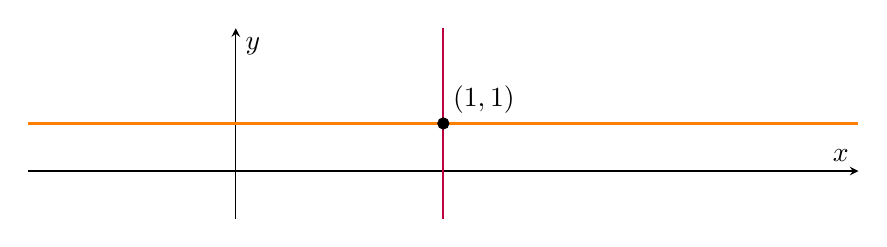
\begin{tikzpicture}
		\begin{axis}[
				width=\linewidth,
				height=4cm,
				axis lines=center,
				xlabel={$x$},
				ylabel={$y$},
				ticks=none,
				xmin=-1, xmax=3,
				ymin=-1, ymax=3,
			]
			\addplot[purple, thick] coordinates {(1,-1) (1,3)};
			\addplot[orange, thick, samples=100, domain=-1:3] (\x,{1});
			\addplot[only marks, mark=*, black] coordinates {(1,1)} node[above right] {$(1,1)$};
		\end{axis}
	\end{tikzpicture}
	\caption{Elementary row operations rotate lines about their solution.}
	\label{fig:ero-rotation}
\end{marginfigure}
Geometrically this has the effect of \emph{rotating} each line about the solution (\cref{fig:ero-rotation}).

\newthought{A more complicated example.} The system represented by the augmented matrix:
\begin{equation*}
	\left[
		\begin{array}{cccc|c}
			1  & 0 & 1 & 3 & 2 \\
			2  & 1 & 2 & 0 & 0 \\
			-1 & 3 & 4 & 0 & 1 \\
		\end{array}
		\right]
\end{equation*}
Following the steps of Gauss-Jordan Elimination, we chose $(1,1)$ to be our pivot:
\begin{equation*}
	\left[
		\begin{array}{cccc|c}
			\boxed{1} & 0 & 1 & 3 & 2 \\
			2         & 1 & 2 & 0 & 0 \\
			-1        & 3 & 4 & 0 & 1 \\
		\end{array}
		\right]
\end{equation*}
We then add multiples of the first row to the second and third rows such that their first entries all become 0.
\begin{equation*}
	\left[
		\begin{array}{cccc|c}
			\boxed{1} & 0 & 1 & 3  & 2  \\
			0         & 1 & 0 & -6 & -4 \\
			0         & 3 & 5 & 3  & 3  \\
		\end{array}
		\right]
	\begin{array}{l}
		\\
		R_2 \iff R_2 - 2R_1 \\
		R_3 \iff R_3 + R_1
	\end{array}
\end{equation*}
We then shift the pivot down and to the right.
\begin{equation*}
	\left[
		\begin{array}{cccc|c}
			1 & 0         & 1 & 3  & 2  \\
			0 & \boxed{1} & 0 & -6 & -4 \\
			0 & 3         & 5 & 3  & 3  \\
		\end{array}
		\right]
\end{equation*}
And add multiples of the second row to the third row so that its second entry becomes 0.
\begin{equation*}
	\left[
		\begin{array}{cccc|c}
			1 & 0         & 1 & 3  & 2  \\
			0 & \boxed{1} & 0 & -6 & -4 \\
			0 & 0         & 5 & 21 & 15 \\
		\end{array}
		\right]
	\begin{array}{l}
		\\
		\\
		R_3 \iff R_3 - 3R_2
	\end{array}
\end{equation*}
Shift the pivot once again:
\begin{equation*}
	\left[
		\begin{array}{cccc|c}
			1 & 0 & 1         & 3  & 2  \\
			0 & 1 & 0         & -6 & -4 \\
			0 & 0 & \boxed{5} & 21 & 15 \\
		\end{array}
		\right]
\end{equation*}
And finally divide the third row by 5 and add multiples of it to the first row such that its third entry becomes 0.
\begin{equation*}
	\left[
		\begin{array}{cccc|c}
			1 & 0 & 0 & -1.2 & -2.2 \\
			0 & 1 & 0 & -6   & -4   \\
			0 & 0 & 1 & 4.2  & 3
		\end{array}
		\right]
	\begin{array}{l}
		R_1 \iff R_1 - R_3 \\
		\\
		R_3 \iff R_3 \div 5
	\end{array}
\end{equation*}
This matrix is in reduced row echelon form and can't be reduced any further. This system has three
\emph{basic}\sidenote[][-1cm]{A variable is \emph{basic} if its column contains the leading entry of a row, otherwise its \emph{non-basic}.
	Consistent systems with more unknowns than equations will always have at least one non-basic variable. All non-basic
	variables are free variables, and all basic variables are linear combinations of constants and non-basic variables.}
variables, $x_1, x_2,$ and $x_3$, and one \emph{non-basic} variable $x_4$. When writing the parametric solution to a system
with free variables, like we have here, it is crucial to always chose the non-basic variables as free. This
leaves us with the following linear equations:
\begin{align*}
	x_1 -1.2x_4  & = -2.2 & \implies & x_1  =-2.2+1.2x_4 \\
	x_2 -6x_4    & = -4   & \implies & x_2  =-4+6x_4     \\
	x_3 + 4.2x_4 & = 3    & \implies & x_3  = 3-4.2x_4
\end{align*}
And so the solution will be:
\begin{equation*}
	S = \{(-2.2+1.2x_4,-4+6x_4,3-4.2x_4,x_4)\text{ | }x_4 \in \mathbb{R}\}
\end{equation*}

\section{Reasoning about Systems of Linear Equations}

\newthought{How can we tell} how many solutions a system has, or if it's consistent at all, just by looking at
its augmented matrix?

If, after completing Gauss-Jordan elimination, one of the leading entries is on the right of the augmenting line,
the system is inconsistent. If a system is consistent and all variables are basic variables, then there is a unique
solution. If the system is consistent and there are any free variables, the system has infinitely many solutions.

\newthought{Examples}
\begin{equation*}
	\underset{\text{Inconsistent}}{
		\left[
			\begin{array}{ccc|c}
				1 & 0 & 1 & 1         \\
				0 & 1 & 2 & 1         \\
				0 & 0 & 0 & \boxed{3}
			\end{array}
			\right]
	}
	\underset{\text{Unique Solution}}{
		\left[
			\begin{array}{ccc|c}
				\boxed{1} & 0         & 1         & 1 \\
				0         & \boxed{1} & 2         & 1 \\
				0         & 0         & \boxed{2} & 3
			\end{array}
			\right]
	}
	\underset{\text{Infinite Solutions}}{
		\left[
			\begin{array}{cccc|c}
				1 & 0 & 1 & \boxed{1} & 2 \\
				0 & 1 & 2 & \boxed{1} & 1 \\
				0 & 0 & 2 & \boxed{3} & 4
			\end{array}
			\right]
	}
\end{equation*}
The first is inconsistent since there is a leading entry after the augmenting line. This says $0x+0y+0z=3$ which
does not make any sense, so there can't be any solutions. The second system doesn't have any leading entries after
the augmenting line and has as many equations as unknowns, so all the variables are basic and there is a unique solution
$(x,y,z)=(-0.5,-2,1.5)$. The third has more unknowns than equations and is consistent, and so one of the variables must
be non-basic and free. Therefore, there is an infinite solution set $S=\{(0.5x_4,2x_4-3,2-1.5x_4,x_4)\text{ | }x_4 \in \mathbb{R}\}$.

\section{Summary}

Solving systems of linear equations quickly and easily is crucial to the study of linear algebra, since so many of the
problems we will face will boil down to a system of linear equations. We can solve systems of linear equations by
first finding the matrix equation \textbf{Ax}$=$\textbf{B}, and the subsequent augmented matrix \textbf{A|B}; then identifying
if the system is consistent by identifying the basic and non-basic variables, and applying elementary row operations with
the method described by Gauss-Jordan elimination. In Chapter 3, we will finally define properly the idea of vector spaces,
and use the tools developed in this chapter to solve various problems related to them.



%Chapter 3 - Vector Spaces and Subspaces
\chapter{Vector Spaces and Subspaces}

\newthought{The concept of a vector space} is fundamental to the study of linear algebra.

\part{Analysis}
\fancyhead[LE]{\textbf{\thepage \quad \textit{Analysis}}}
\part{Quantum Mechanics}
\fancyhead[LE]{\textbf{\thepage \quad \textit{Quantum Mechanics}}}

\bibliography{refs}
\bibliographystyle{plainnat}

\end{document}
